\documentclass[tikz,10pt]{standalone}

\begin{document}
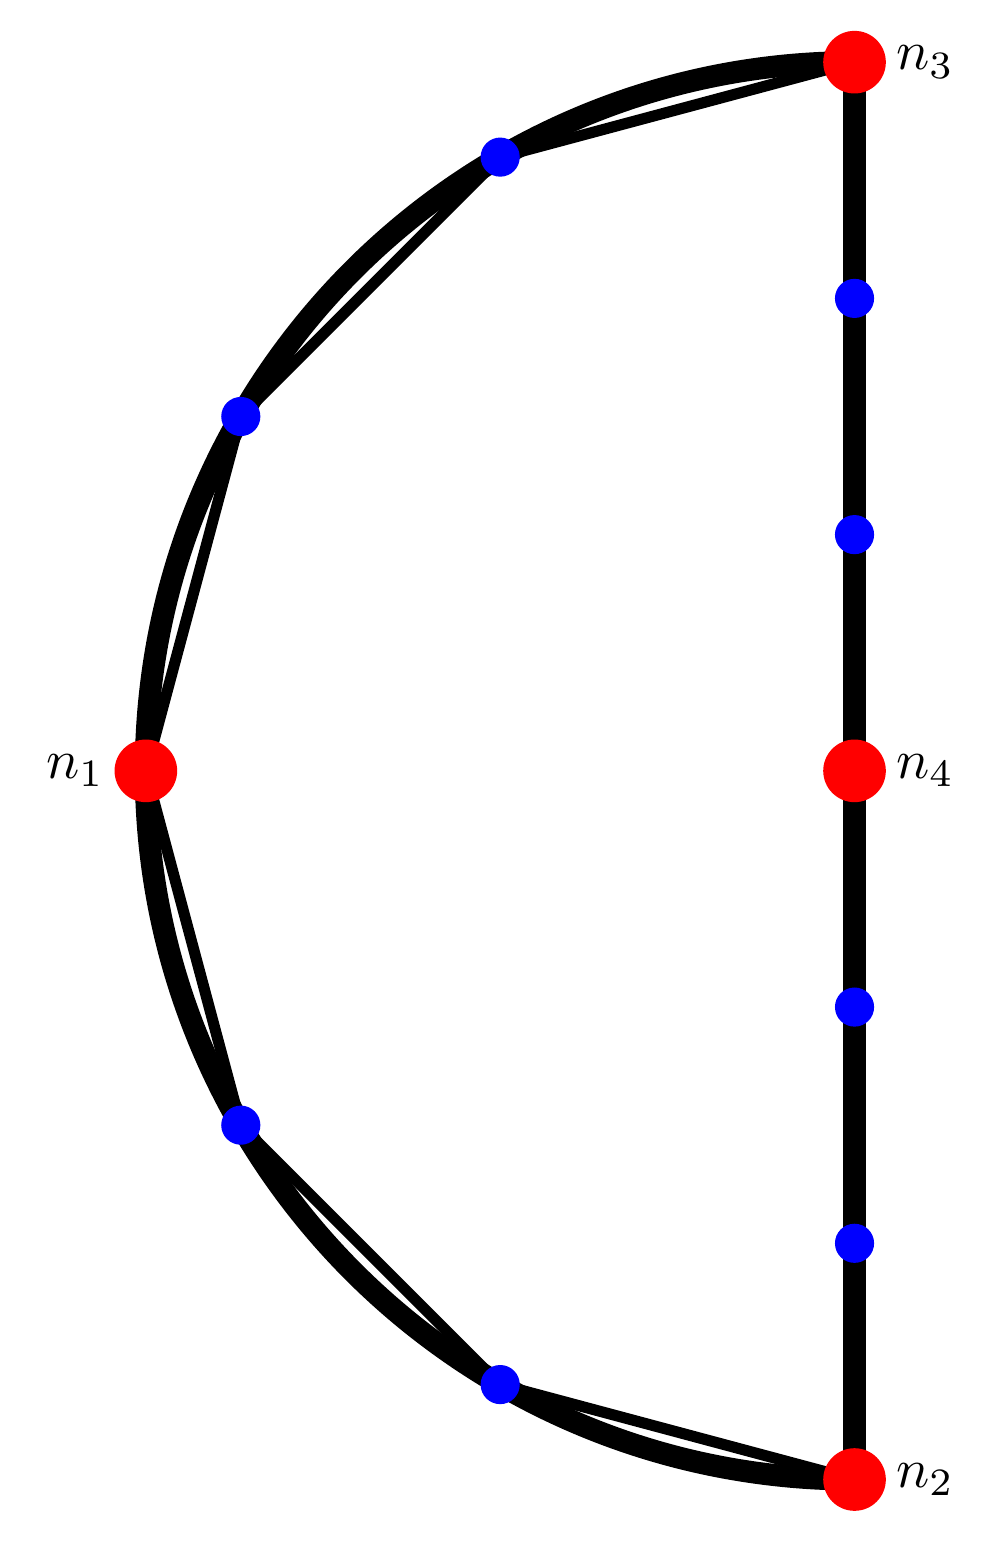
\begin{tikzpicture}

  % Bounding box of the scheme
  \draw (-4,0) node (Bb1) {} ;
  \draw (0,0) node (Bb2) {} ;

  %%%%%%%%%%%%%%%%%%%%%%%%%%%%%%%%% Background of the mesh %%%%%%%%%%%%%%%%%%%%%%%%%%%%%%%%%%%%
  \draw[color=black, line width=8] (0,9) arc [start angle=90, end angle=270, x radius=9cm, y radius=9cm];
  \draw[color=black, line width=8] (0,9) -- (0,-9) ;
  
  %%%%%%%%%%%%%%%%%%%%%%%%%%%%%%%%% Points pour travailler %%%%%%%%%%%%%%%%%%%%%%%%%%%%%%%%%%%%

  % Sommets de blocs
 \draw (-9,0) node (1) {} ;
 \draw (0,-9) node (2) {} ;
 \draw (0,9) node (3) {} ;
 \draw (0,0) node (4) {} ;

 \draw (1) node[scale=2, left = 4pt] {$n_{1}$} ;
 \draw (2) node[scale=2, right = 4pt] {$n_{2}$} ;
 \draw (3) node[scale=2, right = 4pt] {$n_{3}$} ;
 \draw (4) node[scale=2, right = 4pt] {$n_{4}$} ;
 
 % Noeuds sur les arêtes
 \draw ({9*cos(210)},{9*sin(210)}) node (5) {} ;
 \draw ({9*cos(150)},{9*sin(150)}) node (6) {} ;
 \draw ({9*cos(240)},{9*sin(240)}) node (7) {} ;
 \draw ({9*cos(120)},{9*sin(120)}) node (8) {} ;
 \draw ( 0,-6) node (9) {} ;
 \draw ( 0,-3) node (10) {} ;
 \draw ( 0, 3) node (11) {} ;
 \draw ( 0, 6) node (12) {} ;
 
 %%%%%%%%%%%%%%%%%%%%%%%%%%%%%%%%%%%% Arêtes de blocs %%%%%%%%%%%%%%%%%%%%%%%%%%%%%%%%%%%%%
 \draw[line width=4] (1) -- (6) ;
 \draw[line width=4] (6) -- (8) ;
 \draw[line width=4] (8) -- (3) ;
 
 \draw[line width=4] (1) -- (5) ;
 \draw[line width=4] (5) -- (7) ;
 \draw[line width=4] (7) -- (2) ;

 %%%%%%%%%%%%%%%%%%%%%%%%%% Points sur les noeuds et sommets %%%%%%%%%%%%%%%%%%%%%%%%%%%%%%%
 % Sommets de blocs
 \foreach \i in {1,2,...,4} {
   \draw (\i) node[circle, fill=red, inner sep=8pt] {} ;
 }

 % Noeuds sur des arêtes de blocs
 \foreach \i in {5,6,...,12} {
   \draw (\i) node[circle, fill=blue, inner sep=5pt] {} ;
 }

 

\end{tikzpicture}
\end{document}
